\subsection{对数 GLSM 不变量}%
\label{sub:Log GLSM invariants}

\begin{defn}
    我们将对数映射 \(f\) 的\textit{装饰热带型}（decorated tropical type）定义为
    \[ \bm{\tau} = (G, c \colon \H \to \Z, \beta \colon \V \to H_2(X)). \]
\end{defn}

\begin{defn}
    一个对数映射或穿孔映射 \(f\) 称为\textit{紧致型}（compact type）的，如果
    \begin{enumerate}
        \item \(\Ima \Sigma(f)_t\) 对所有 \(t\) 都有界；
        \item 对所有接触阶为 \(0\) 的半边 \(h\) 有 \(f(p_h) \in 0_{\mf{P}}\)。
    \end{enumerate}
\end{defn}

现在我们可以定义范畴 \(\mc{R}(\mf{P}, \tau)\)，它由纤维在 fs 对数概形范畴 \(\ms{LogSch}\) 之上、以 \(\tau\) 标记的稳定穿孔 R-映射组成。

\begin{thm}[{\cite{CJR2021,CJRpunctured}}]
    叠 \(\mc{R}(\mf{P},\bm{\tau})\) 由一个带基本/最小对数结构的真 DM叠代表。
\end{thm}

\begin{rmk}
    若 \(\V = \ab\{v\}\) 为单点集，则我们记
    \[ \mc{R}_{g, c}(\mf{P}, \beta) \coloneqq \mc{R}(\mf{P}, \bm{\tau}). \]
\end{rmk}

考虑下图
\begin{equation*}
\begin{tikzcd}
    & \mf{P} \ar{d} \\
    \mc{C} \ar{ur}{f} \ar{d}{\pi} \ar{r} & B \C_{\omega}^{\times} \\
    \mc{R},
\end{tikzcd}
\end{equation*}
其中我们置 \(\mc{R} \coloneqq \mc{R}(\mf{P}, \bm{\tau})\)。于是完美障碍理论由
\[ T_{\mc{R}/\ms{Log}_{\mf{M}_G}} \to \E_{\square} = R \pi_* f^* T_{\mf{P}/B\C_{\omega}^{\times}}. \]
定义。这里两个切丛均指对数切复形。由完美障碍理论，这定义了典范虚类
\[ [\mc{R}(\mf{P}, \bm{\tau})]^{\vir}. \]
这个虚类的主要缺点是它不能重现 Gromov–Witten 理论。不过，我们可以考察它与 GW 理论的差别，但这需要一个双有理修正。设 \(Q\) 为尖幺半群。它有一个偏序：\(a < b\) 是指存在非零 \(c \in Q\) 使得 \(a+c = b\)。

\begin{defn}
    我们称 \(f\) 或 \(\Sigma(f)\) 具有\textit{一致极大退化}（uniform maximal degeneracy），如果存在 \(e_{\max} \in \ab\{e_v \mid v \in \V \}\) 使得对所有 \(v \in \V\) 有 \(e_{\max} \geq e_v\)。
\end{defn}

\begin{rmk}
    若 \(f\) 为紧致型且具有一致极大退化，则 \(\Sigma(f)\) 被 \(e_{\max}\) 一致有界。
\end{rmk}

\begin{defn}
    定义 \(\mc{U}(\mf{P}, \bm{\tau})\) 为以 \(\bm{\tau}\) 标记且具有一致极大退化的稳定穿孔或对数 R-映射的叠。
\end{defn}

\begin{rmk}
    若 \(\V = \ab\{v\}\) 为单点集，则我们记
    \[ \mc{U}_{g, c}(\mf{P}, \beta) \coloneqq \mc{U}(\mf{P}, \bm{\tau}). \]
    若某个接触阶为负，则我们记
    \[ \mc{U}_{g, c}(\infty, \beta) \coloneqq \mc{U}(\mf{P}, \bm{\tau}). \]
\end{rmk}

注意到顶点分为两类：若顶点映到 \(0\)，则或者至少有一条半边向上指，或者所有接触阶均为 \(0\)，此时全部收缩。这些称为\textit{对数顶点}（log vertex）。另一类顶点是不映到 \(0\) 的顶点：或者所有半边都向下指，或者有一些半边向上指。这些称为\textit{\(\infty\)-顶点}。此外，紧致型的顶点即那些没有向上指半边的顶点。

若忘掉一致极大退化这一条件，则有一个态射
\[ \mc{U}(\mf{P}, \bm{\tau}) \xrightarrow{F} \mc{R}(\mf{P}, \bm{\tau}) \]
它是 \(\ms{LogSch}\) 上的子范畴。然而，作为代数叠之间的态射，它是对数 étale、真且满射的。此外，\(\mc{U}\) 具有由 \(\mc{R}\) 拉回的典范完美障碍理论。当顶点集为单点集时，我们有
\begin{align*}
    F_* [\mc{U}_{g, c}(\mf{P}, \beta)]^{\vir} &= [\mc{R}_{g, c}(\mf{P}, \beta)]^{\vir}; \\
    F_* [\mc{U}_{g, c}(\infty, \beta)]^{\vir} &= [\mc{R}_{g, c}(\infty, \beta)]^{\vir}.
\end{align*}
在对数顶点的情形，我们实际上有从带 p-场的稳定映射模空间出发的包含
\begin{equation*}
\begin{tikzcd}
    \mc{U} \ar{rr}{F} & & \mc{R} \\
    & \mc{R}_{g,c}(\mf{P}^{\circ}, \beta) \ar[hookrightarrow]{ul} \ar[hookrightarrow]{ur}.
\end{tikzcd}
\end{equation*}
若记 p-场的模空间为 \(\mc{R}^{\circ}\)，则边界
\[ \Delta \coloneqq \mc{U} \setminus \mc{R}^{\circ} \]
是一个 Cartier 除子。由一致极大退化的条件，我们有一个截面
\[ e_{\max} \in H^0(\bar{M}_{\mc{U}}). \]
这等价于一个态射
\[ \mc{U} \to ([\A^1/\G_m], 0) \]
的数据，它将 \(0\) 拉回为 \(\Delta\)。

我们将\textit{超势}（superpotential）定义为一个函数
\begin{equation*}
\begin{tikzcd}
    \mf{P}^{\circ} \ar{rr}{W} \ar{dr} && \mc{L}_{\omega} \ar{dl} \\
    & B \C_{\omega}^{\times}.
\end{tikzcd}
\end{equation*}
其\textit{临界轨迹}（critical locus）记为
\[ \on{Crit}(W) = (\d{W} = 0). \]
我们称 \(W\) 具有\textit{真临界轨迹}，若 \(\on{Crit}(W) \to B\C_{\omega}^{\times}\) 是真（proper）的。

例如，假设我们对 GW 理论感兴趣。设 \(X\) 为光滑射影簇，\(V\) 为 \(X\) 上的向量丛，\(s \in H^0(V)\)。令 \(Z = (s = 0)\)。于是我们得到
\[ W \colon \mf{P}^{\circ} = V^{\vee} \boxtimes \mc{L}_{\omega} \xrightarrow{s \otimes 1_{\omega}} \mc{L}_{\omega}. \]

\begin{lem}
    \(W\) 具有真临界轨迹当且仅当 \(Z\) 光滑且余维数为预期值。
\end{lem}

\begin{exm}
    设 \(X\) 为一点，\(V = \C\)，且 \(s \neq 0\)。则 \(\d{W} = s \neq 0\)，故临界轨迹为空。
\end{exm}

利用 Kiem–Li 的余截面局部化方法~\cite{KiemLi2013}，我们可以得到一个虚类
\[ [\mc{R}_{g, c=n}(\mf{P}^{\circ}, \beta)]_W^{\vir}, \]
它支撑在临界轨迹上。在 GW 理论中，它等于 GW 虚类
\[ \pm [\bar{M}_{g,n}(\on{Crit}(W), \beta)]^{\vir}, \]
其中符号可以显式算出。

\begin{thm}[{\cite{CJR2021,CJW2021}}]
    设 \(\bm{\tau}\) 为紧致型。在紧致型情形下，
    \begin{enumerate}
        \item \(\mc{U}(\mf{P}, \bm{\tau})\) 具有约化完美障碍理论，由此得到约化虚类 \([\mc{U}(\mf{P}, \bm{\tau})]^{\vir}\)；
        \item \(\Delta\) 具有约化完美障碍理论，由此得到约化虚类 \([\Delta]^{\vir}\)；
        \item 在单个对数顶点的情形，我们有 \([\mc{U}_{g, c=n}(\mf{P}, \beta)]^{\on{red}} = \pm [\bar{M}_{g,n}(\on{Crit}(W), \beta)]^{\vir}\)。此外还有公式
            \[ [\mc{U}_{g, c=n}(\mf{P}, \beta)]^{\on{red}} = [\mc{U}_{g, c=n}(\mf{P}, \beta)]^{\vir} - \tilde{r} [\Delta]^{\on{red}}, \]
            其中 \(\tilde{r}\) 是 \(W\) 沿 \(\infty\) 的极点阶。
    \end{enumerate}
\end{thm}

\subsection{热带分解与有限生成}%
\label{sub:Tropical decomposition and finite generation}

下文的热带分解及其应用取自工作文稿~\cite{CJRtropical2025}。有效不变量及其公理在~\cite{CJRpunctured} 中发展。

从现在起，我们考虑一个更简单的设定：\(X\) 是光滑射影簇而 \(V\) 是 \(X\) 上的线丛。此时我们假设 \(Z = (s = 0)\) 是余维 \(1\) 的光滑子簇。进一步假设 \(Z\) 是 Calabi–Yau 三维簇。我们考虑不变量
\[ N_{g, \beta} \coloneqq \int_{[\bar{M}_{g,0}(Z, \beta)]^{\vir}} 1 \in \Q \]
与生成级数
\[ F_g = \sum_{\beta \geq 0} N_{g, \beta} Q^{\beta} \in \Lambda \coloneqq \C \ps{Q}. \]

\begin{conj}[Yamaguchi-Yau, Alim-L\"ange {\cite{YY2004,AlimLange2007}}]
    假设 \(Z\) 满足 \(g=0\) 镜像对称。则存在有限生成的 \(\Q\)-代数 \(R \subset \Lambda\)，使得对所有 \(g \geq 2\) 有 \(F_g \in (I_0(q))^{2g-2} R\)。
\end{conj}

我们的主要目标如下。

\begin{thm}[{\cite{CJRtropical2025}}]
    设 \(Z\) 是 Fano 四维簇 \(X\) 中的 Calabi–Yau 三维超曲面，且 \(X\) 无奇上同调。设 \(\{\phi_j\}\) 是 \(H^*(X)\) 的一组基，\(\ab\{\phi^j\}\) 为对偶基。则对所有 \(g \geq 0\)，我们有
    \begin{align*}
        &F_g = (-1)^{1-g} \sum_{\tau' \in G_g'} \frac{(-1)^{\abs{\V_{\infty}}}}{\abs{\Aut(\tau')}} \cdot \prod_{E \in \E} c(E) \\
        & \cdot \sum_{j_E \mid E = \ab\{E_{\log}, E_{\infty}\} \in \E} \prod_{\substack{v \in \V_{\infty} \\ g(v)=1 \\ \H_v = \ab\{E_{\infty}\}}} c_1^{\mr{eff}}(\phi^{j_E}) \cdot \prod_{\substack{v \in \V_{\infty} \\ g(v) \geq 2}} \tilde{Q}^{\beta(v)} \cdot \exp \ab(\int_{\beta(v)} K(Q) )  \\
        & \cdot \ab(\prod_{E_{\infty} \in \H_v'}\int_{\beta(v)} \phi^{j_E}) \cdot c_{g(v), \beta(v)}^{\on{eff}} 
         \cdot \prod_{v \in \V_{\log}} \Omega_{g(v), \abs{\H_1(v)}, \abs{\H_2(v)}} (\phi_{j_E} \colon E_{\log} \in \H_1(v)).
    \end{align*}
\end{thm}

\begin{exm}
    设 \(Y\) 为带其环面对数结构的环面簇。则 \(\Sigma(Y)\) 是视为锥复形的环面扇，我们可以考虑其边界 \(\Delta_Y = \sum_{\rho \in \Sigma(Y)^1} \Delta_{\rho}\)。
\end{exm}

若我们考虑 \([\Delta]^{\on{red}}\)，应当得到类似的公式
\[ [\Delta]^{\on{red}} = \sum_{\rho \in \Sigma(\Delta)(1)} [\Delta_{\rho}]^{\on{red}}. \]
现在的问题是 \(\rho\) 代表什么。事实上，它们参数化刚性热带曲线。在热带化
\begin{equation*}
\begin{tikzcd}
    \Sigma(C)_{\rho} \ar{d} \ar{r} & \Sigma(\mc{C}) \ar{r}{f} \ar{d} & \R_{\geq 0} \\
    \rho \ar[hookrightarrow]{r} & \Sigma(\mc{U}),
\end{tikzcd}
\end{equation*}
中，我们看到 \(f_{\rho}\) 是刚性的当且仅当源热带曲线是一个二部图，其中一组顶点映到 \(e_{\max}\) 而另一组顶点映到 \(0\)。

\begin{exm}
    设 \(X\) 为一点且 \(Z = \emptyset\)。再考虑 \(g = 2, n = 0\)。此时可能的图如~\Cref{fig:tropgraphs} 所示。
    \begin{figure}[htpb]
    \begin{center}
    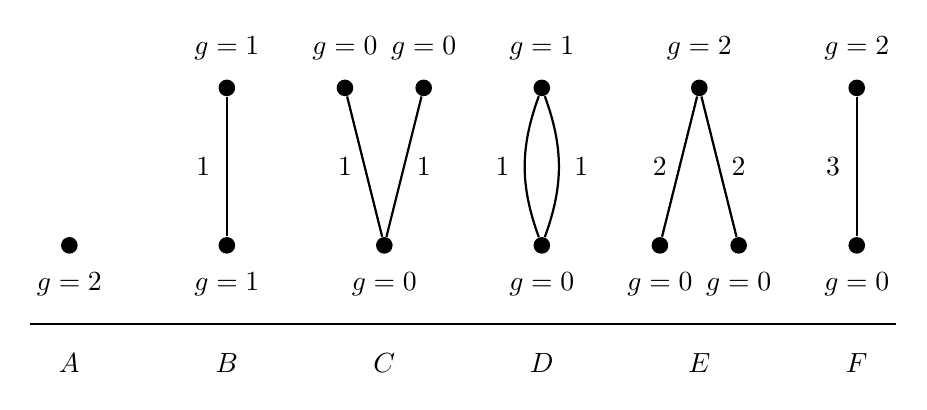
\begin{tikzpicture}[scale=1, transform shape]
        \node[fill=black,circle,minimum size=6pt,inner sep=0pt] (A) at (0,0) {};
        \node[fill=black,circle,minimum size=6pt,inner sep=0pt] (B1) at (2,0) {};
        \node[fill=black,circle,minimum size=6pt,inner sep=0pt] (B2) at (2,2) {};
        \node[fill=black,circle,minimum size=6pt,inner sep=0pt] (C1) at (4,0) {};
        \node[fill=black,circle,minimum size=6pt,inner sep=0pt] (C2) at (3.5,2) {};
        \node[fill=black,circle,minimum size=6pt,inner sep=0pt] (C3) at (4.5,2) {};
        \node[fill=black,circle,minimum size=6pt,inner sep=0pt] (D1) at (6,0) {};
        \node[fill=black,circle,minimum size=6pt,inner sep=0pt] (D2) at (6,2) {};
        \node[fill=black,circle,minimum size=6pt,inner sep=0pt] (E1) at (8,2) {};
        \node[fill=black,circle,minimum size=6pt,inner sep=0pt] (E2) at (7.5,0) {};
        \node[fill=black,circle,minimum size=6pt,inner sep=0pt] (E3) at (8.5,0) {};
        \node[fill=black,circle,minimum size=6pt,inner sep=0pt] (F1) at (10,0) {};
        \node[fill=black,circle,minimum size=6pt,inner sep=0pt] (F2) at (10,2) {};
        \draw[-,thick] (B1) -- (B2);
        \draw[-,thick] (C2) -- (C1) -- (C3);
        \draw[-,thick] (D1) edge[bend left=20] (D2);
        \draw[-,thick] (D2) edge[bend left=20] (D1);
        \draw[-,thick] (E2) -- (E1) -- (E3);
        \draw[-,thick] (F1) -- (F2);
        \node at (0,-0.5) {$g=2$};
        \node at (2,-0.5) {$g=1$};
        \node at (4,-0.5) {$g=0$};
        \node at (6,-0.5) {$g=0$};
        \node at (7.5,-0.5) {$g=0$};
        \node at (8.5,-0.5) {$g=0$};
        \node at (10,-0.5) {$g=0$};
        \node at (2,2.5) {$g=1$};
        \node at (3.5,2.5) {$g=0$};
        \node at (4.5,2.5) {$g=0$};
        \node at (6,2.5) {$g=1$};
        \node at (8,2.5) {$g=2$};
        \node at (10,2.5) {$g=2$};
        \draw[-,thick] (-0.5,-1) -- (10.5,-1);
        \node at (0,-1.5) {$A$};
        \node at (2,-1.5) {$B$};
        \node at (4,-1.5) {$C$};
        \node at (6,-1.5) {$D$};
        \node at (8,-1.5) {$E$};
        \node at (10,-1.5) {$F$};
        \node at (1.7,1) {$1$};
        \node at (3.5,1) {$1$};
        \node at (4.5,1) {$1$};
        \node at (5.5,1) {$1$};
        \node at (6.5,1) {$1$};
        \node at (7.5,1) {$2$};
        \node at (8.5,1) {$2$};
        \node at (9.7,1) {$3$};
    \end{tikzpicture}
    \end{center}
        \caption{当 $g=2$ 时 $X = \mr{pt}$、\(Z = \emptyset\) 的热带型的图。}%
    \label{fig:tropgraphs}
    \end{figure}
\end{exm}

\begin{thm}[热带量子莱夫谢茨 {\cite{CJRtropical2025}}]
    设 \(X\) 与 \(Z\) 同前。对任意 \(\beta \in H_2(X)\)、\(\alpha_1, \ldots, \alpha_n \in H^*(X)\) 以及 \(k_1, \ldots, k_n \in \N\)，我们有
    \begin{align*}
        \int_{[\bar{M}_{g,n}(Z,\beta)]^{\vir}} \prod_{j=1}^n \ev_j^* (\alpha_j) \psi^{k_j}={}& (-1)^{1-g+\beta \cdot Z} \cdot \sum_{\tau \vdash (g,n,\beta)} \frac{(-1)^{\abs{\V_{\infty}}}}{\abs{\Aut(\tau)}} \cdot \prod_{E \in \E} c(E) \\
        & \cdot \sum_{\ab\{j_E \mid E = \ab\{E_{\log}, E_{\infty}\}\}}  \prod_{v \in \V_{\infty}} \int_{[\mc{U}_v]^{\on{red}}} \prod_{E_{\infty} \in \H_v} \ev_{E_{\infty}}^* \phi^{j_E}  \\
        &  \cdot \prod_{v \in \V_{\log}} \int_{[\mc{R}_v]^{\vir}} \prod_{E_{\log}} \ev_{E_{\log}}^* (\phi_{j_E}) \cdot \prod_{h \in \L_v} \ev_h^* \alpha_h \cdot \psi_h^{k_h} .
    \end{align*}
\end{thm}

\begin{rmk}
    还有一个虚局部化公式，已在~\cite{CJRlocalization} 中宣布，它既可应用于约化理论（仅有 R-环面作用），也可应用于典范理论（可应用于环境空间的全部自同构）。
\end{rmk}

现在考虑一个 \(\infty\)-顶点。令 \(\tau_v = (g, c, \beta)\)，并令 \(\mc{U}_v = \mc{U}_{g,c}(\infty, \beta)\)。第一个计算是
\begin{align*}
    \on{red}\dim \mc{U}_v &= \chi(f^* T_{\mf{P}/B \C^{\times}_{\omega}}) + 1 + \on{trop}\dim  \\
    &= \vir\dim \bar{M}_{g,n}(Z, \beta) + \sum_{h \in \H } (c(h) + 1),
\end{align*}
其中热带维数为 \(3g-4+n\)。注意到所有接触阶都是负的，故第二项至多为零。特别地，我们已经证明了
\begin{cor}[{\cite{CJRpunctured}}]
    若 \(\vir\dim \bar{M}_{g,n}(Z,\beta) < 0\)，则 \([\mc{U}_v]^{\on{red}} = 0\)。
\end{cor}
我们还有一个\textit{平衡条件}（balancing condition），它断言
\begin{equation}\label{eqn:balancing condition}
    \sum_{h \in \H} c(h) = \deg f^* \mc{O}(\infty) = \int_{\beta} c_1(V) - (2g-2+n).
\end{equation}
这可以改写为
\[ 0 \geq \sum_{h \in \H} (c(h)+1) = \int_{\beta} c_1(V) - (2g-2). \]
\begin{prop}[{\cite{CJRpunctured}}]
    我们看到在下列情形下 \(\infty\)-顶点不存在：
    \begin{enumerate}
        \item \(g = 0\) 且 \(V\) 为 nef；
        \item \(g=1\) 且 \(V\) 为丰富，除非 \(\beta = 0\) 且所有 \(c(h) = -1\)。
    \end{enumerate}
\end{prop}

\begin{defn}
    一个标记称为\textit{单位}（unit），若其接触阶为 \(-1\)。
\end{defn}

\begin{notn}
    我们以 \(\1\) 记单位扇区，并记 \(\tau_{v+\1} = (g, c+\1, \beta)\)、\(\mc{U}_{v+\1} = \mc{U}_{g, c+\1}(\infty, \beta)\) 以及 \(\mc{R}_{v+\1} = \mc{R}_{g, c+\1}(\infty, \beta)\)。
\end{notn}

\begin{thm}[{\cite[Theorems~1.16--1.17]{CJRpunctured}}]\leavevmode
    \begin{enumerate}
        \item 存在态射 \(F_{\1} \colon \mc{U}_{v+\1} \xrightarrow{s} \mc{C}^{\circ} \xrightarrow{\pi} \mc{U}_v\)，其中 \(s\) 是双有理的；
        \item 约化虚类满足等式 \(s_* [\mc{U}_{v+\1}]^{\on{red}} = \pi^* [\mc{U}_v]^{\on{red}}\)；
        \item 若 \(D\) 是 \(X\) 上的除子，则 \(F_{\1 *} (\ev_{\1}^* D \cap [\mc{U}_{v+\1}]^{\on{red}}) = \ab(\int_{\beta} D) [\mc{U}_v]^{\on{red}}\)；
        \item 考虑下图
            \begin{equation*}
            \begin{tikzcd}
                \mc{U}_{v+\1} \ar{r}{F} \ar{d}[swap]{F_{\1}} & \bar{M}_{g,n+1} \ar{d}[swap]{p} \\
                \mc{U}_v \ar{r}{F} & \bar{M}_{g,n}.
            \end{tikzcd}
            \end{equation*}
            则 \(F_* [\mc{U}_{v+\1}]^{\on{red}} = p^* F_* [\mc{U}_v]^{\on{red}}\)。
    \end{enumerate}
\end{thm}

\begin{exm}
    考虑 \(g = 1\) 且 \(Z_d \subset X = \P^N\) 为超曲面的设定。我们只需考虑 \(\beta = 0\) 且对所有 \(h \in \H\) 有 \(c(h) = -1\) 的情形。于是我们看到
    \[ \prod_h \ev_h^* \alpha_h \cdot [\mc{U}_{1,c}(\infty,\beta)]^{\mr{red}} = \ev_{h^{\star}}^* \ab(\prod_h \alpha_h) \cap [\mc{U}_{1,\1}(\infty,\beta)]^{\on{red}}. \]
\end{exm}

\begin{prop}[{\cite{CJRpunctured}}]
    我们实际上有
    \[ \mc{U}_{1,\1}(\infty, 0) \simeq \mc{R}_{1,\1}(\infty, 0) \]
    以及等式
    \[ [\mc{U}_{1,\1}(\infty, 0)]^{\on{red}} = c_{\dim X} \ab(\mc{H}^{\vee} \boxtimes T_{\mf{P}/B\C_{\omega}^{\times}} + \mc{O} - V). \]
\end{prop}

\begin{exm}
    现在考虑五次三维簇 \(Z_5 \subset \P^4\)。于是我们看到 \(\on{red}\dim \mc{U}_v = \sum_{h \in \H} (c(h)+2)\)。单位公理把我们归约到 \(c(h) \leq -2\) 的情形。现在我们必须确定当所有 \(c(h) = -2\) 时需要考虑的新不变量的个数，这等价于求可能的 \(\beta\) 的个数。平衡条件断言
    \begin{align*}
        \sum_{h \in \H} c(h) &= \int_{\beta} c_1(V) - (2g-2+n) \\
        &= 5\beta - (2g-2+n),
    \end{align*}
    由此可得 \(0 \geq \sum (c(h)+1) = 5\beta - (2g-2)\)，从而 \(\beta \leq \frac{2g-2}{5}\)。\footnote{这恰好是我们假设有限生成、全纯反常方程、轨形正则性以及 conifold 间隙条件时所预测的未知数个数。}
\end{exm}

\begin{conj}[Janda {\cite[Conjecture~1.6]{CJRtropical2025}}]\leavevmode
    \begin{enumerate}
        \item 我们有 \(K(Q) = \log I_0(q) \cdot c_1(K_X^{\vee}) - \frac{I_1}{I_0}\) \\
        \item 典范理论满足 \(\Omega \in I_0(q)^{2g-2+2n_1 + 3 n_2} \cdot R\)。
    \end{enumerate}
\end{conj}

\begin{cor}[{\cite[Theorem~1.7]{CJRtropical2025}}]
    关于 \((X, V)\) 的上述猜想蕴含 \(Z\) 的 Yamaguchi–Yau 有限生成。
\end{cor}

